% -*- TeX:de -*-
\NeedsTeXFormat{LaTeX2e}
\documentclass[12pt,a4paper]{article}
\usepackage[german]{babel} % german text
\usepackage[DIV12]{typearea} % size of printable area
\usepackage[T1]{fontenc} % font encoding
%\usepackage[latin1]{inputenc} % most likely on Windows
\usepackage[utf8]{inputenc} % probably on Linux
\usepackage{multicol}

% PLOTTING
\usepackage{pgfplots} 
\usepackage{pgfplotstable}
\usepackage{url}
\usepackage{graphicx} % to include images
\usepackage{tikz}
\usepackage{subfigure} % for creating subfigures
\usepackage{amsmath} % a bunch of symbols
\usepackage{amssymb} % even more symbols
\usepackage{booktabs} % pretty tables

% a floating environment for circuits
\usepackage{float}
\usepackage{caption}

%\newfloat{circuit}{tbph}{circuits}
%\floatname{circuit}{Schaltplan}

% a floating environment for diagrams
%\newfloat{diagram}{tbph}{diagrams}
%\floatname{diagram}{Diagramm}

\selectlanguage{german} % use german

\begin{document}

%%%%%%% DECKBLATT %%%%%%%
\thispagestyle{empty}
			\begin{center}
			\Large{Fakultät für Physik}\\
			\end{center}
\begin{verbatim}


\end{verbatim}
							%Eintrag des Wintersemesters
			\begin{center}
			\textbf{\LARGE WS 2013/14}
			\end{center}
\begin{verbatim}


\end{verbatim}
			\begin{center}
			\textbf{\LARGE{Physikalisches Praktikum\\ für das Bachelorstudium}}
			\end{center}
\begin{verbatim}




\end{verbatim}

			\begin{center}
			\textbf{\LARGE{PROTOKOLL}}
			\end{center}
			
\begin{verbatim}





\end{verbatim}

			\begin{flushleft}
			\textbf{\Large{Experiment (Nr., Titel):}}\\
							%Experiment Nr. und Titel statt den Punkten eintragen
			\LARGE{PW4 Oberflächenspannung, Viskosität, Hygrometrie, Schmelzwärme}	
			\end{flushleft}

\begin{verbatim}

\end{verbatim}	
							%Eintragen des Abgabedatums, oder des Erstelldatums des Protokolls
			\begin{flushleft}
			\textbf{\Large{Datum:}} \Large{31.10.2013}
			\end{flushleft}
			
\begin{verbatim}
\end{verbatim}
							%Namen der Protokollschreiber
		\begin{flushleft}
			\textbf{\Large{Namen:}} \Large{Patrick Braun, Johannes Kurz}
			\end{flushleft}

\begin{verbatim}


\end{verbatim}
							%Kurstag und Gruppennummer, zb. Fr/5
			\begin{flushleft}
			\textbf{\Large{Kurstag/Gruppe:}} \Large{DO/2}
			\end{flushleft}

\begin{verbatim}



\end{verbatim}
							%Name des Betreuers, das Praktikum betreute.
			\begin{flushleft}
			\LARGE{\textbf{Betreuer:}}	\Large{ Franz Sachslehner }	
			\end{flushleft}

%%%%%%% DECKBLATT ENDE %%%%%%%
\pagebreak
\setlength{\columnsep}{20pt}
\begin{multicols}{2}
\section{Einleitung}

\section{Oberflächenspannung}


% Regress in Strich gegen N
%%%B (y-intercept) = -1,343535761669278e-04 +/- 4,628591085282343e-05
%%%A (slope) = 2,149302255457725e-03 +/- 1,174365191704868e-05

Bevor Messungen durchgeführt werden können muss die verwendete Waage geeicht werden. Dazu werden auf die Schale 0.1g schwere Metallstücke gelegt und die dazugehörigen Striche abgelesen. Dadurch kann die Kraft pro Strich errechnet werden.
$$F = m * a$$
Bei einem Verhältnis von $1g \approx 4.56 Strich$ welches durch lineare Regression der Messwerte zu erhalten ist, entspricht ein Strich \textbf{K = 0.00N}.\\
Durch
Literaturwert: Wasser bei $20^{\circ}$ 72,75 mN/m\\


Eichgewichter, Pinzette, Waage, Schale mit Wasser, Metallring\\

\subsection{Messwerte und Ergebnisse}
%\begin{figure}[H]
%	\centering
%	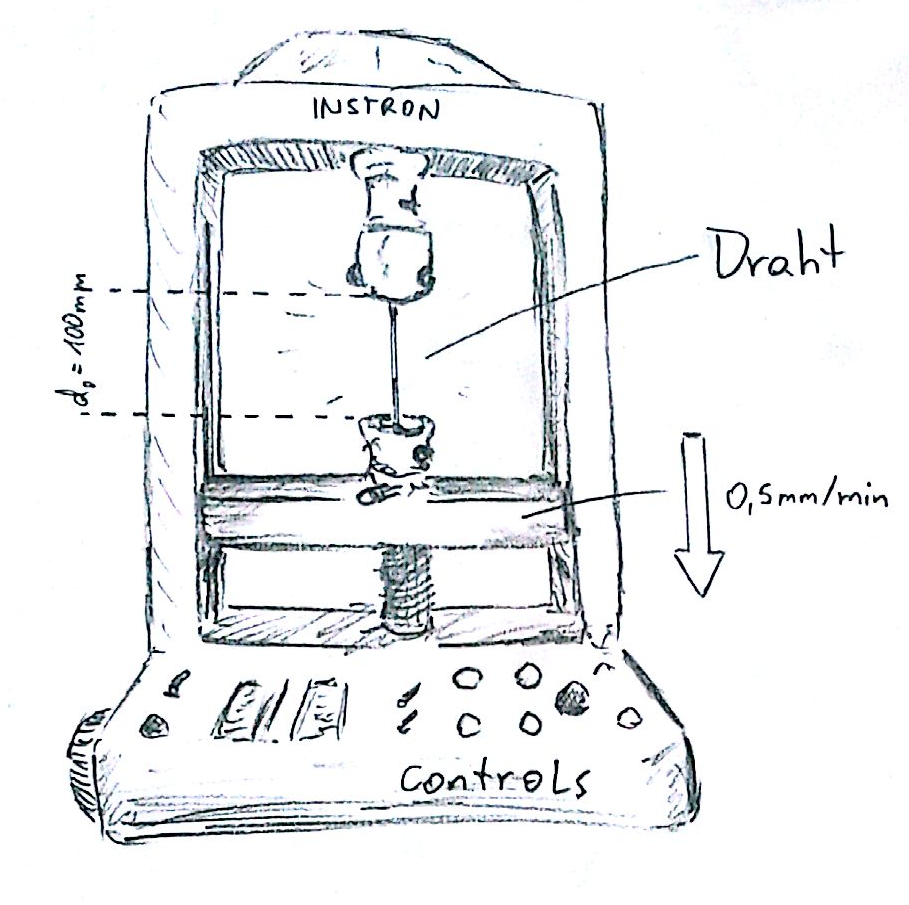
\includegraphics[scale=0.23]{./figure/zugversuch_aufbau.png}
%	\caption{Skizze Versuchsaufbau}
%	\label{fig:elastizitaet}
%\end{figure}
%\noindent

\begin{figure}[H]
	\centering
	\pgfplotstabletypeset[
			columns={g,strich},
			col sep=tab,
			columns/T1/.style={column name=$T_1[s]$},
			columns/T2/.style={column name=$T_2[s]$},
			every head row/.style={before row=\hline,after row=\hline\hline},
			every last row/.style={after row=\hline},
			every first column/.style={
								column type/.add={|}{}
							        },
			every last column/.style={
								column type/.add={}{|}
								}
			]{./data/oberflaechenspannung_eichung.dat}
	\caption{Eichungsmessung der Waage}
	\label{fig:oberflaeche_eichung}
\end{figure}
\noindent

strich
39
38
39
39
39
39
40
%#Neues Wasser destiliert
47
46
46
46
46

%#35


24.00mm +- 0.05mm\\
23.15mm +- 0.05mm\\
\\
Erste:\\
$23.5^{\circ}C$\\
Zweite:\\
$22.3^{\circ}C$\\
\subsection{Diskussion}


%%%%%%%%%%%%%%%%%%%%%%%%%%%%%%%%%%%%
\section{Viskosität}
Rühre, Pinzette, Kugeln
Thermometer Sumit DT150\\
\subsection{Messwerte und Ergebnisse}
Temp: $24^{\circ}C \pm 1^{\circ}C$\\
Länge Innen-Innen: 13.42cm\\
Dichte Flüssigkeit: $1225 \pm 5 kg/m^2$\\
\\
Messungen 1:\\
$0.794 \pm 0.002mm$\\
$16.1 \pm 0.1 mg$\\

Fallzeiten:\\
2.4s\\
2.37s\\
2.4s\\
2.38\\
2.41\\
2.41\\
2.31\\
2.44\\
2.47\\
2.44\\
2.47\\
\\
Messung 2:\\
$6.6 \pm 0.1mg$\\
$0.595 \pm 0.01mm$\\
\\
Fallzeiten:\\
3.94\\
3.97\\
3.97\\
4.13\\
3.97\\
3.97\\
3.97\\
3.79\\
3.97\\
3.88\\
4.04\\
\\
\textbf{Höppler-Viskosimeter}\\
HAAKE, Thermometer, Heizgerät\\
Temperatur: $25.0^{\circ}C \pm 0.1^{\circ}C$\\
Messung 1: 2m51s90ms\\
Messung 2: 2m51s32ms\\
Messung 3: 2m51s32ms\\
\\
Temperatur: $50.6^{\circ}C \pm 0.1^{\circ}C$\\
Messung 1: 0m42s25ms\\
Messung 2: 0m41s63ms\\
Messung 3: 0m41s78ms\\
\\
\subsection{Diskussion}


%%%%%%%%%%%%%%%%%%%%%%%%%%%%%%%%%%%%
\section{Luftfeuchtigkeit}
\subsection{Messwerte und Ergebnisse}
$T_{Start} = 24^{\circ}C \pm 1^{\circ}C$\\

\subsection{Diskussion}


%%%%%% EIS - SCHMELZWAERME %%%%%%%%

\section{Schmelzwärme vonEis}
Bei der Wärmezufuhr in einen Stoff kommt es bei Phasenübergängen zu Zeiten konstanter Temperatur, währendderer die zugeführte Energie zur Gänze in die Zustandsänderung, nicht jedoch in die Temperaturänderung geht.\\
\\
In diesem Versuch soll die spezifische Schmelzwärme von Eis (Wasser aus der Haushaltsleitung, Wien) bestimmt werden. Es wird dazu die Mischungsmethode verwendet:\\
In einem (idealerweise völlig) wärmeisolierten Gefäß werden 2 Stoffe unterschiedlicher Temperatur gemischt. Die abgegebene Wärmemenge des wärmeren Stoffes muss wegen der Energieerhaltung gleich der aufgenommenen Wärmemenge des kälteren und des Gefäßes sein.\\
Aus den Anfangstemperaturen und der Mischtemperatur lässt sich beispielsweise auf die latente Wärme schließen, die beim Schmelzvorgang von Eis frei wird.
$$\Delta Q_1=(C_k+m_wc_w)(T_1-T_m)=$$
$$=\Delta Q_2 = m_eS+m_ec_w(T_m-T_S)$$
$S$ ist die gesuchte spezifische Schmelzwärme des Eises, die Massen $m_e$, $m_w$ des verwendeten Wasser und Eises sowie die Wärmekapazitäten $c_w$, $C_k$ von Wasser und dem verwendeten Gefäß gehen in die Rechnung ein.\\

\noindent Equipment:
\begin {itemize}
	\item Ein Kalorimetergefäß mit Rührer
	\item Wasser und Eis
	\item Ein ULab-Datalogger mit Temperatursonde
\end {itemize}

Das Kalorimeter wird, zu etwas mehr als der Hälfte, mit erhitztem Wasser (ca. $80^{\circ}$ C) gefüllt und der Temperaturverlauf des Systems wird mehrere Minuten gemessen.\\
Nach ein paar Minuten wird Eis eingebracht (weniger als Wasser). Es ist darauf zu achten, das Eis schnell einzuwerfen und sofort und durchgehend zu rühren um den Schmelzvorgang zu beschleunigen.\\
Schließlich soll ein instantaner Temperaturausgleich approximiert werden.\\
Während des gesamten Versuchs wird der Temperaturverlauf gemessen, der grob in 3 Abschnitte geteilt werden kann, die durch Anlegen von Geraden idealisiert werden (vgl. Abb. \ref{fig:Tempverlauf-Eis}):\\
- Vor der Zugabe von Eis\\
- während des Schmelzvorganges\\
- nach der Vermischung


\end{multicols}

%%%% Diagramm Eis
\begin{figure}[H]
	\centering
	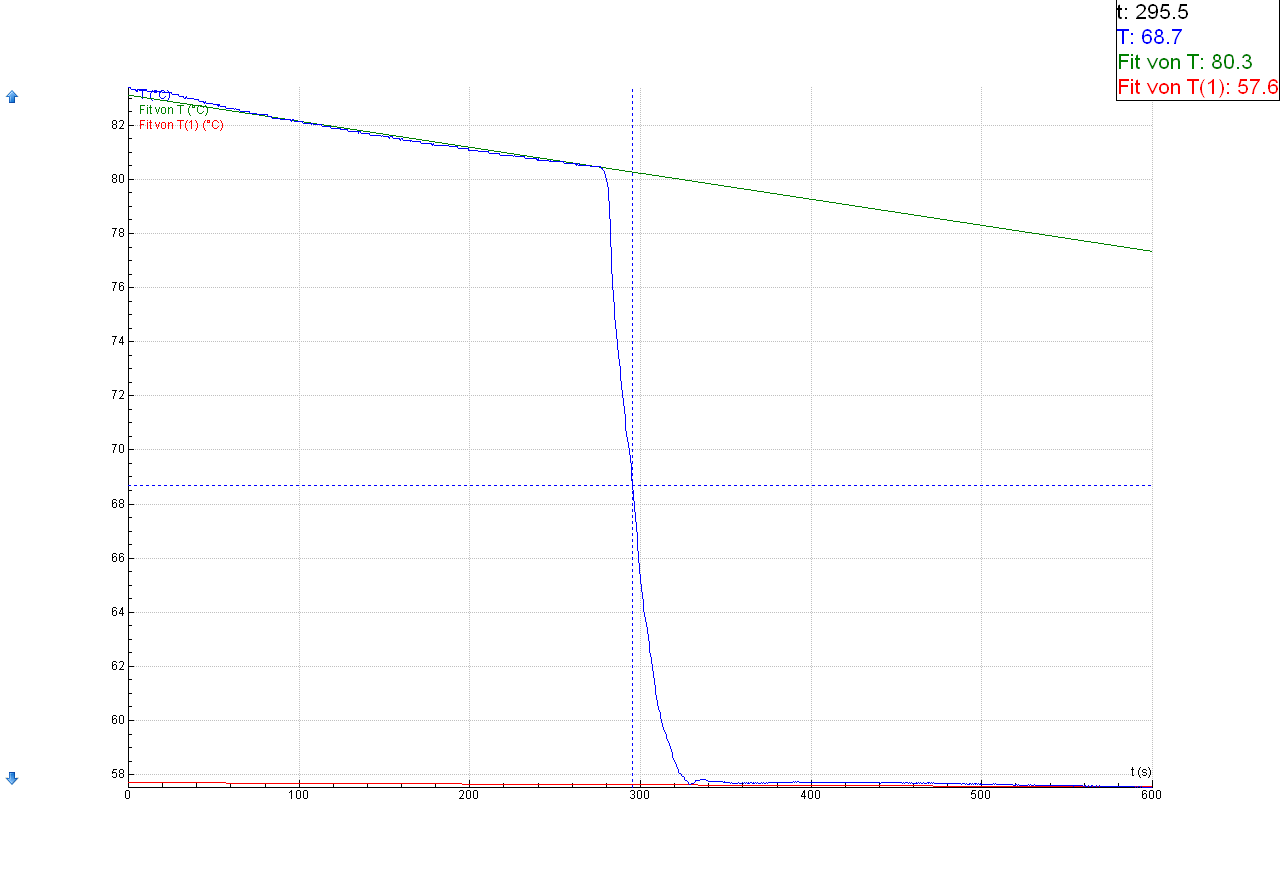
\includegraphics[scale=0.35]{./figure/PW4_graph.PNG}
	\caption{Temperatur in [$^\circ$C] gegen die Zeit in [s] im Kalorimeter\ }
	{\centering Screenshot aus Coach6}
	\label{fig:Tempverlauf-Eis}
\end{figure}
\noindent

\begin{multicols}{2}


\subsection{Messwerte und Ergebnisse}

\begin{itemize}
	\item Wärmekapazitäten:\\
	Kalorimeter: $C_k = (100 \pm 10) J/K$\\
	Wasser (20$^{\circ}$C): $c_w=(4,182) J/gK$
	
	\item Massen:\\
	Kalorimeter: $(236.6 \pm 0.1)g$\\
	Wasser: $m_w = (154.0 \pm 0.2)g$\\
	Eis: $m_e = (26.0 \pm 0.2)g$
	
	\item Temperaturen:\\
	Anfang: $T_1=(80 \pm 0.5) ^\circ C$\\
	Ende: $T_m=(58 \pm 0.5) ^\circ C$\\
	Schmelztemp. Eis: $T_S = 0 ^\circ C$
\end{itemize}

\noindent spezifische Schmelzwärme von Wasser:\\
$$S =(387 \pm   ) kJ/kg$$

\subsection{Diskussion}

\section{Quellen}
Formeln und Abbildung Fahrradpendel:\\
\url{http://www.univie.ac.at/anfpra/neu1/pw/pw3/PW3.pdf}\\

\noindent spezifische Wärmekapazität von Wasser:\\
\url{http://de.wikipedia.org/wiki/Spezifische_W%C3%A4rmekapazit%C3%A4t}

\end{multicols}
\end{document}